\section{Introduction}

Urban PM$_{2.5}$ remains one of the most important environmental health risks in cities because it penetrates deeply into the respiratory system, contributes to cardiovascular and pulmonary disease, and often varies strongly across space and time \citep{WHO2021, Pope2006, Burnett2018, Cohen2017}. In rapidly urbanizing tropical megacities, this challenge is intensified by dense traffic, mixed land use, seasonal stagnation, and complex local source patterns. Bangkok is a particularly important case because it experiences recurrent haze episodes and pronounced short-term variability in air quality, while also facing continuing challenges in PM$_{2.5}$ management \citep{Aman2020, Narita2019, ChooChuay2020, Kanchanasuta2020}. Parks are often assumed to provide air-quality benefits, yet the extent to which they actually buffer PM$_{2.5}$ exposure, and the conditions under which they do so most effectively, remain insufficiently resolved \citep{Janhall2015, Diener2021, Abhijith2017, Venter2024}.

Most studies evaluating the air-quality role of urban parks rely on static comparisons, such as mean concentrations measured inside and outside green spaces, or on short-duration field campaigns that emphasize average differences over limited time windows \citep{Pugh2012, Su2022, Yin2019}. Although these approaches are useful for establishing whether a park may be cleaner than its surroundings on average, they cannot resolve the temporal structure of pollution dynamics. In particular, they do not distinguish whether a park suppresses short-lived spikes, moderates diurnal oscillations, or attenuates broader multi-day episodes. They also cannot clearly separate two fundamentally different behaviors: reducing fluctuation amplitude versus remaining synchronized with the surrounding urban signal. As a result, parks that differ substantially in their temporal buffering behavior may still appear similar when judged only by mean PM$_{2.5}$ levels.

A wavelet-based perspective offers a way to address this limitation. Continuous wavelet transform (CWT) analysis decomposes a time series into timescale-specific components \citep{Torrence1998, Cazelles2008}, making it possible to examine how strongly different temporal rhythms are expressed across hourly, diurnal, and multi-day bands. For paired park--outside PM$_{2.5}$ data, this yields two complementary descriptors: attenuation, which reflects the extent to which variability is damped in the park relative to its outside comparator, and coherence, which reflects the extent to which the two locations remain dynamically coupled at a given timescale \citep{Grinsted2004}. This framework is especially attractive for urban air pollution because it moves beyond a single mean-difference metric and asks a more informative question: which temporal components of PM$_{2.5}$ are buffered by parks, and which remain closely tied to the broader urban environment? Wavelet-based approaches have also been used in broader air-pollution and environmental time-series analysis to investigate scale-dependent relationships with meteorological forcing and other controls \citep{Li2014}.

A second unresolved issue is why some parks appear to perform better than others. Simple greenness indicators such as the Normalized Difference Vegetation Index (NDVI) \citep{Tucker1979} can serve as useful first approximations, but they do not adequately represent the structural context in which a park operates. PM$_{2.5}$ buffering is likely to depend not only on how green a park is on average, but also on how that vegetation is arranged relative to surrounding built surfaces, whether a protected interior core exists, how abrupt the park edge is, and whether nearby water or other land-cover elements modify local microclimatic conditions \citep{Vos2013, Wania2012, Barwise2020, Hewitt2020, Zhou2019}. In other words, park performance is likely to be relational and spatially structured rather than reducible to a single mean greenness value. Yet this more layered explanatory framework has been less commonly tested against timescale-specific PM$_{2.5}$ behavior.

Accordingly, this study addresses two linked objectives. First, it quantifies timescale-specific PM$_{2.5}$ attenuation and coherence between paired park-interior and outside monitoring stations in Bangkok during 2021 using a continuous wavelet transform framework. Second, it investigates whether differences in wavelet behavior across parks are associated with spatially explicit explanatory features, including ring-gradient land-cover contrast, water-related context, and park morphology. The analysis is intentionally framed as a 2021 case study because this year provides the most defensible full-year pairing after rigorous quality gating of station completeness and overlap. The study area, station distribution, and retained Tier-A park--outside pairs are shown in Fig.~\ref{fig:study_area_map}.

\begin{figure}[htbp]
\centering
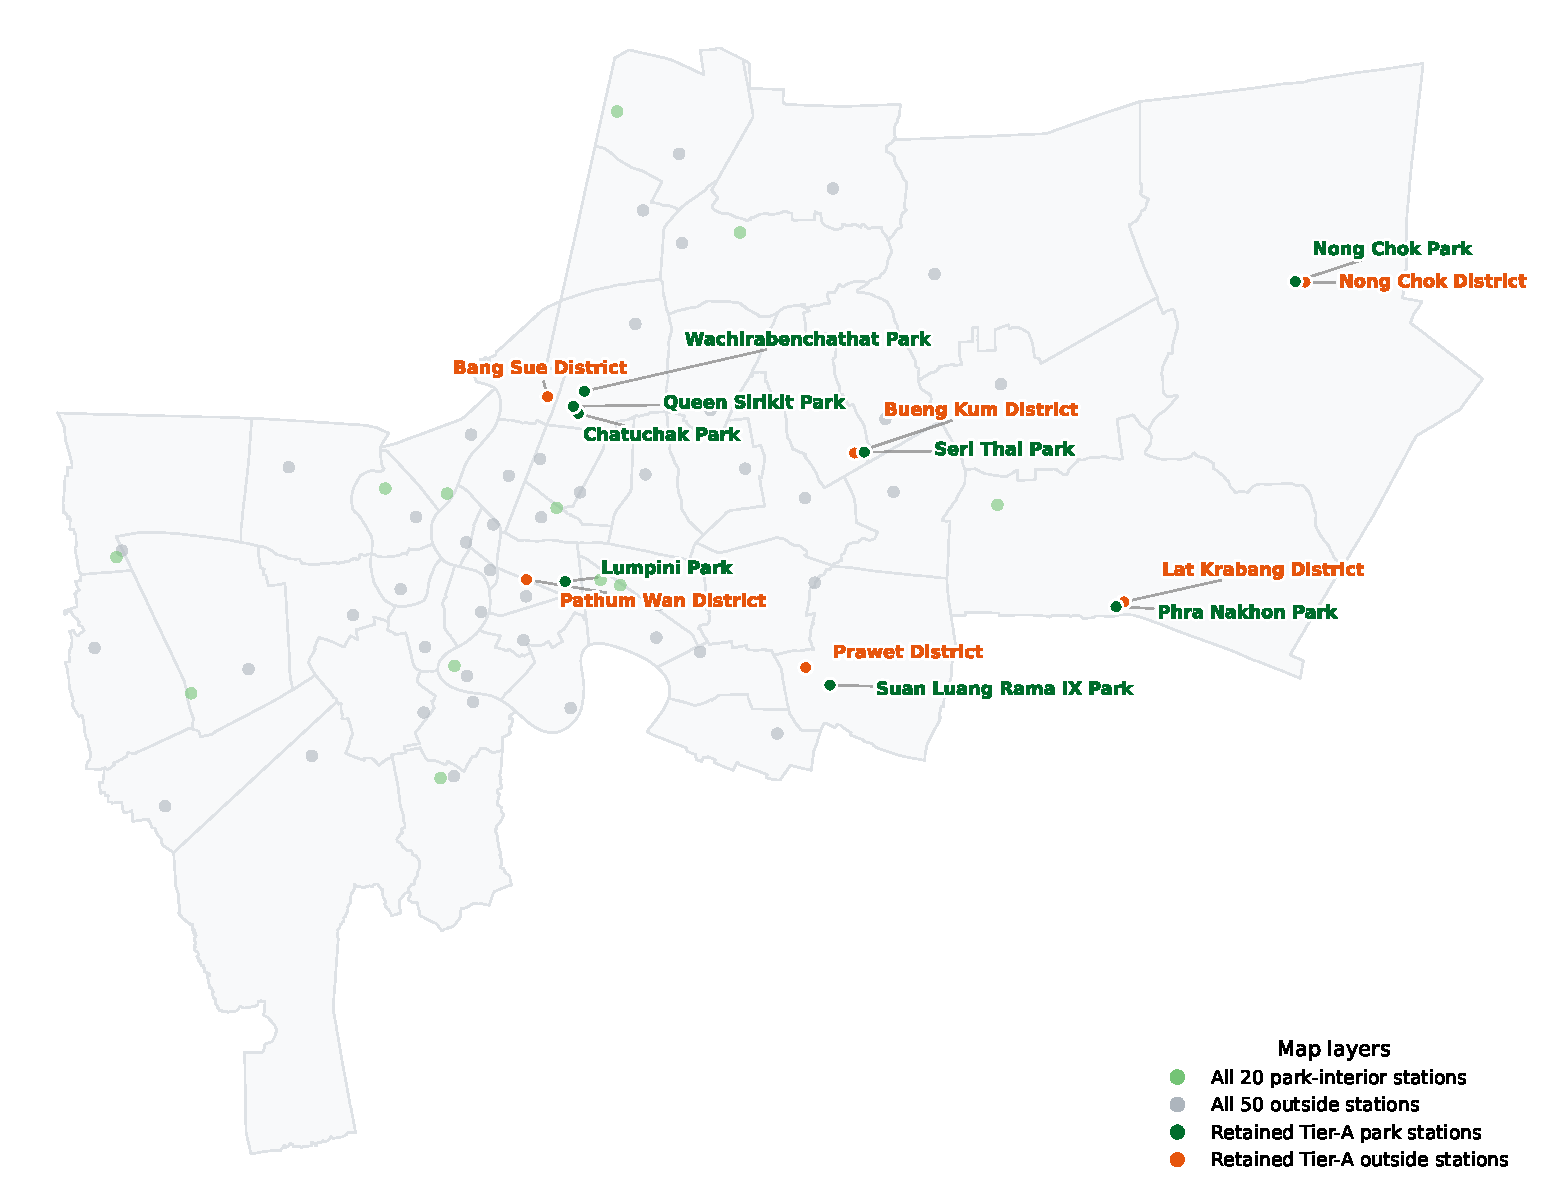
\includegraphics[width=\textwidth]{figures/Fig1_study_area_map.pdf}
\caption{Study area map of Bangkok showing the 20 park-interior PM$_{2.5}$ monitoring stations, the 50 district-level outside stations, and the eight retained Tier-A park--outside pairs used in the defensible 2021 wavelet analysis.}
\label{fig:study_area_map}
\end{figure}

The main contribution of this study is therefore methodological as well as substantive. It presents a transparent wavelet attenuation--coherence framework for paired urban PM$_{2.5}$ series under strict data-quality control, demonstrates that parks can be grouped into distinct damping regimes rather than treated as a single homogeneous class, and explores a layered explanatory hierarchy that extends beyond mean greenness to annulus-based land-cover gradients, water context, and morphology. By doing so, the study reframes the role of urban parks from a simple question of whether they reduce PM$_{2.5}$ on average to a more nuanced question of which parks buffer which temporal rhythms, how strongly they remain coupled to surrounding urban dynamics, and what spatial characteristics are most consistently associated with those outcomes.